\documentclass[12pt,oneside]{book}
\usepackage{geometry}                		% See geometry.pdf to learn the layout options. There are lots.
\geometry{a4paper}                   			% ... or a4paper or a5paper or ... 
%\geometry{landscape}                		% Activate for for rotated page geometry
%\usepackage[parfill]{parskip}    		% Activate to begin paragraphs with an empty line rather than an indent
\usepackage{graphicx}				% Use pdf, png, jpg, or epsß with pdflatex; use eps in DVI mode
								% TeX will automatically convert eps --> pdf in pdflatex		
\usepackage{amssymb}

\usepackage[spanish]{babel}			% Permite que partes automáticas del documento aparezcan en castellano.
\usepackage[utf8]{inputenc}			% Permite escribir tildes y otros caracteres directamente en el .tex
\usepackage[T1]{fontenc}				% Asegura que el documento resultante use caracteres de una fuente apropiada.

\usepackage{hyperref}				% Permite poner urls y links dentro del documento

\title{Lenguajes de Programacion \\ Librillo de Reportes de Proyectos.}
\author{José Velez \\ Carlos Ramirez \\Keyla Figueroa}
%\date{}							% Activate to display a given date or no date

\begin{document}
\maketitle
\tableofcontents



\chapter{Prefacio}

Este librillo pretende mostrar los objetivos, los problemas presentados en el transcurso del curso de Lenguajes de Programación,
en el desarrollo de los distintos proyectos planteados, mostrar las ventajas y desventajas de las distintas herramientas empleadas
para el desarrollo de las aplicaciones propuestas, las particularidades y como se resolvió los problemas presentados en la implementación de cada aplicación. \ \\ \\ 
Por otro lado, también brinda un resumen de las experiencias en cada herramienta aprendida a lo largo de Curso de Lenguajes de Programación. \ \\ \\
Con el fin de aprovechar al máximo la información de este documento, se explica y se detalla la utilidad de cada herramienta utilizadas
tanto para programar, el control de versionamiento y documentación de las aplicaciones desarrolladas.


\chapter{Introducción}

El Curso de Lenguajes de Programación dictado en Término I -2013 por el Ing. Xavier Tibau, 
pretende obtener como resultados, conocer la sintaxis y semantica de los lenguajes de programación.
Entender el rol del hardware en la implementacion semantica del lenguaje.
Comprender la gramatica de los lenguajes para poder comparar sus caracteristicas y escoger
el lenguaje mas apropiado para una aplicación.
Escribir programas utilizando cada lenguaje de diferentes paradigmas que permitan demostrar
sus caracteristicas y similitudes.




\chapter{Proyecto 1}

\ \\ El proyecto de Qt sudoku fue desarrollado en C++ QT.\ \\



\begin{figure}[htbp]
\begin{center}

\includegraphics[width=.70\textwidth]{./imagenes/qt_logo.png}
\caption{qt}
\label{qt}
\end{center}
\end{figure}



El objetivo del primer Proyecto del Curso de Lenguajes de Programaci\'on fue desarrollar un Sudoku, en QT como herramienta de desarrollo junto a Git como herramienta de versionamiento y el uso de doxygen como herramienta de documentaci\'on.



\ \\
\newpage

\section{Requerimientos del Proyecto Qt Sudoku:}
\ \\ 

Implementar una aplicaci\'on de Sudoku en Qt, en la cual podamos validar si la resoluci\'on de un tablero es v\'alida o no es v\'alida.

\ \\ 

Nuestra aplicaci\'on debe generar tableros de sudoku con distintas dificultades.

\ \\ 

Nuestra aplicaci\'on debe mostrarnos ayuda durante la resoluci\'on del tablero mostr\'andonos, cuando un n\'umero ingresado es incorrecto si ya existe en la misma fila, columna o cuadrante

\ \\ 

Nuestra aplicaci\'on debe ofrecernos la opci\'on de mostrar pistas, la cual nos indicar\'a si los numeros ingresados son correctos o incorrectos validando el tablero.

\ \\ 

Nuestra aplicaci\'on nos permitir\'a llevar un registro de los mejores puntajes obtenidos al resolver el tablero en sus diferentes dificultades.

\ \\


\begin{figure}[htbp]
\begin{center}
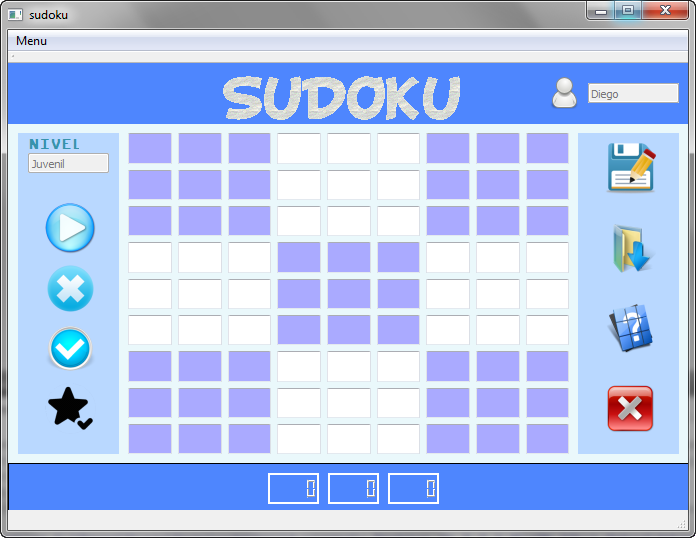
\includegraphics[width=.60\textwidth]{./imagenes/Sudoku.png}
\caption{Tablero Sudoku}
\label{Tablero Sudoku}
\end{center}
\end{figure}


\newpage
\section{Herramientas Utilizadas en el Desarrollo del Proyecto:}

\begin{figure}[htbp]
\begin{center}
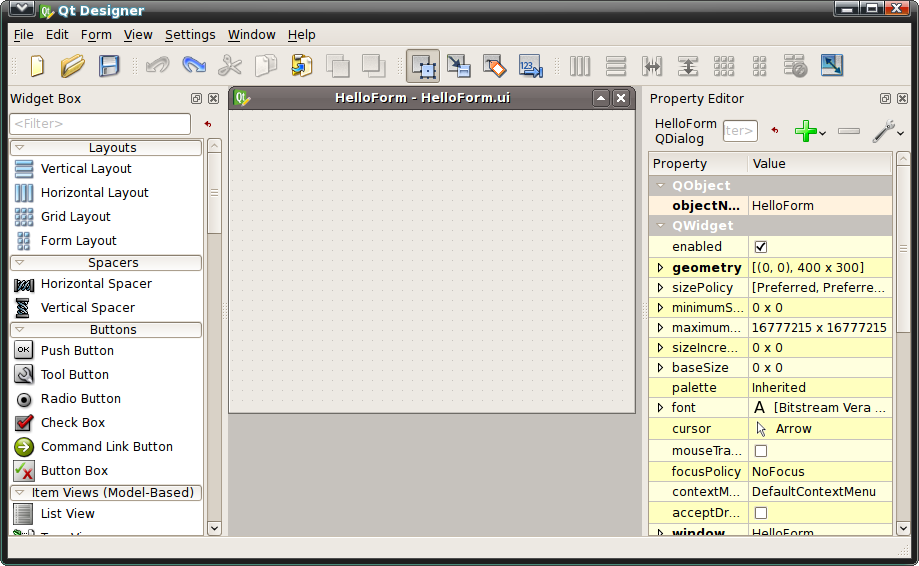
\includegraphics[width=.70\textwidth]{./imagenes/qt.png}
\caption{qt}
\label{qt}
\end{center}
\end{figure}

\ \\ 
Qt es una biblioteca multiplataforma ampliamente usada para desarrollar aplicaciones con interfaz gr\'afica de usuario, asi como tambi\'en para el desarrollo de programas sin interfaz gr\'afica, como herramientas para la linea de comandos y consolas para servidores.
Qt es desarrollada como un software libre y de c\'odigo abierto a trav\'es de Qt Project, donde participa tanto la comunidad, como desarrolladores de Nokia, Digia y otras empresas. Anteriormente, era desarrollado por la divisi\'on de software de Qt de Nokia, que entro en vigor despu\'es de la adquisici\'on por parte de Nokia de la empresa noruega Trolltech, el productor original de Qt, el 17 de junio de 2008.3 Qt es distribuida bajo los terminos de GNU Lesser General Public License (y otras). Por otro lado, Digia est\'a a cargo de las licencias comerciales de Qt desde marzo de 2011.
\ \\


\newpage
\section{GitHub:}
\begin{figure}[htbp]
\begin{center}

\includegraphics[width=.70\textwidth]{./imagenes/github_logo.jpg}
\caption{git}
\label{git}
\end{center}
\end{figure}

\ \\ 
GitHub es una forja para alojar proyectos utilizando el sistema de control de versiones Git. Utiliza el framework Ruby on Rails por GitHub, Inc. (anteriormente conocida como Logical Awesome).
Desde enero de 2010, GitHub opera bajo el nombre de GitHub, Inc.
El c\'odigo se almacena de forma publica, aunque tambi\'en se puede hacer de forma privada, creando una cuenta de pago.
\ \\


\newpage
\section{Doxygen:}
\begin{figure}[htbp]
\begin{center}
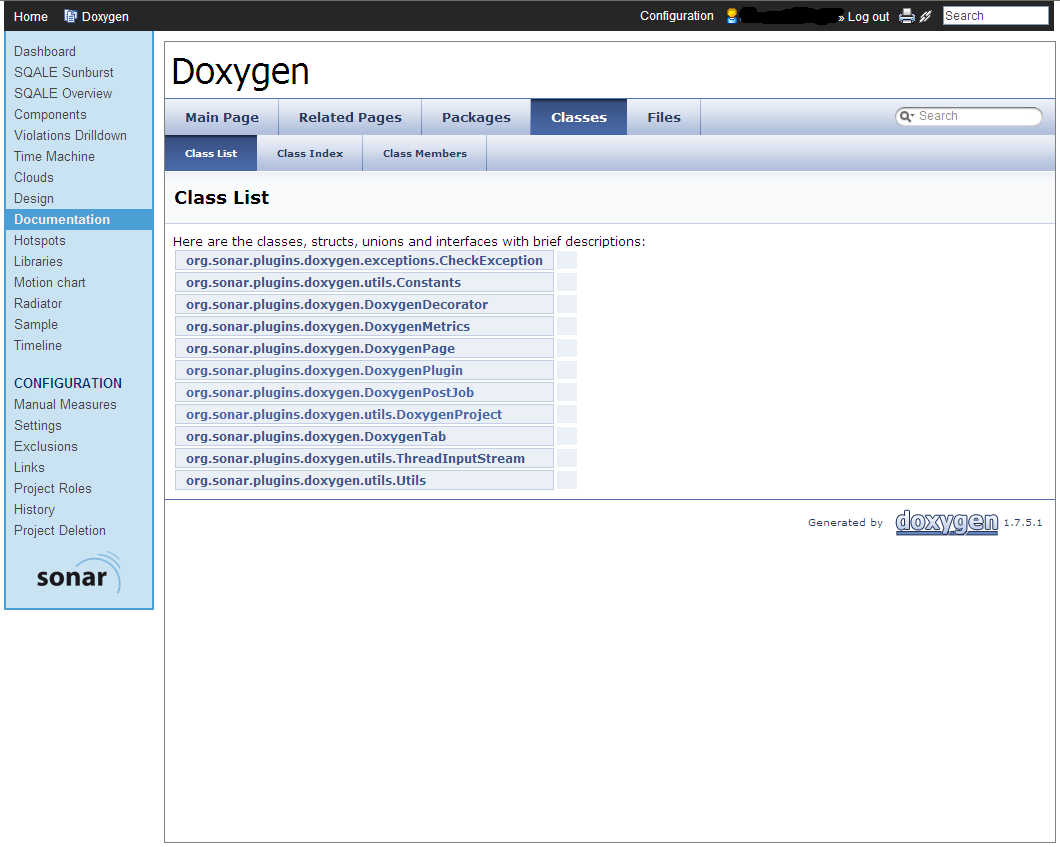
\includegraphics[width=.70\textwidth]{./imagenes/doxygen.png}
\caption{doxygen}
\label{doxygen}
\end{center}
\end{figure}
\ \\ 
Doxygen es un generador de documentaci\'on para C++,C, Java, Objective-C, Python, IDL (versiones Corba y Microsoft), VHDL y en cierta medida para PHP y D. Dado que es f\'acilmente adaptable, funciona en la mayor\'\i{}a de sistemas Unix asi como en Windows y Mac OS X. La mayor parte del c\'odigo de Doxygen esta escrita por Dimitri van Heesch.
Doxygen es un acr\'onimo de dox(document) gen(generator), generador de documentaci\'on para codigo fuente.
Varios proyectos como KDE usan Doxygen para generar la documentacion de su API. KDevelop incluye soporte para Doxygen.
\ \\

\newpage
\section{Objetivos:}
\ \\ 
Crear una aplicaci\'on de sudoku.
\ \\ 
Utilizar QT como principal herramienta de desarrollo.
\ \\ 
Entender el funcionamiento de los signals y slots en QT.
\ \\ 
Implementar la aplicaci\'on con la metodolog\'\i{}a Orientada a objetos.
\ \\ 
Utilizar GIT como herramienta de control de versionamiento.
\ \\ 
Utilizar Doxygen para documentacion del c\'odigo.
\ \\

\section{Desarrollo:}
\ \\ 
El desarrollo de este primer proyecto se realiz\'o entre los tres integrantes del grupo, empezando por crear la interfaz de la aplicaci\'on, como primer paso crear un tablero implementado con una matriz de QtextEdit .

El trabajo fue dividido entre los tres integrantes del grupo,  Diego Cabrera desarrollo la interfaz y la documentaci\'on de la aplicaci\'on. 

La funcionalidad fue dividida entre Carlos Ram\'\i{}rez y Jos� V\'elez.

Jos\'e V\'elez desarrollo el iniciar partida el cual generaba tableros a partir de una plantilla otra de las funcionalidades implementadas fue el cargar y guardar partida, debidamente encriptado con operaciones de desplazamiento al c\'odigo ASCII de los valores del tablero de sudoku. Tambi\'en se encargo de implementar los puntajes que se calculaba en base al tiempo tomado en resolver el juego.

Carlos Ram\'\i{}rez se encargo de implementar la validaci\'on del tablero lleno si era correcto o incorrecto, tambi\'en de la parte de correcci\'on in game de los n\'umeros ingresados en el tablero por medio del evento textChanged y de la opci\'on de dar pista que permit\'\i{}a mostrar al usuario que valor ingresado era correcto y cual no lo era antes de terminar de llenar el tablero.
\ \\

\newpage
\section{Conclusiones:}
\ \\ 
La experiencia en QT, como herramienta de trabajo fue satisfactoria debido a que se orientaba a objetos, y su f\'acil entendimiento por la organizaci\'on al crear las clases y manejar la funcionalidad por medio de los signals y slots, que nos permit�an conectar un evento o cambio de estado en un objeto con una determinada funci\'on de la aplicaci\'on.
El uso de la herramienta GIT es muy importante en el desarrollo de aplicaciones en grupo, ya que nos permite tener una referencia de la colaboraci\'on de cada integrante, y una manera organizada de realizar cambios a nuestra aplicaci�n llevando un registro ordenado de las versiones realizadas a lo largo del proceso de desarrollo.
\ \\ 
\section{Referencias:}
\ \\ 

	http://www.zonaqt.com

\ \\ 

	http://git-scm.com/book/es
\ \\ 

	http://www.stack.nl/~dimitri/doxygen/manual/
	
\ \\ 
\newpage

\chapter{Proyecto 2}
\ \\ El proyecto de Pysudoku fue desarrollado en Python.\ \\



\begin{figure}[htbp]
\begin{center}

\includegraphics[width=.70\textwidth]{./imagenes/python.jpg}
\caption{qt}
\label{qt}
\end{center}
\end{figure}



El objetivo del segundo Proyecto del Curso de Lenguajes de Programaci\'on fue cambiar de lenguaje nuestro sudoku en QT a Python, en Python que se encontro cambio en la sintaxis instrucciones, un lenguaje mas estructurado por identaciones y una particularidad en el uso de variables se continu\'o trabajando junto a Git como herramienta de versionamiento y el uso de doxygen como herramienta de documentaci\'on.



\ \\
\newpage

\section{Requerimientos del Proyecto PySudoku:}
\ \\ 

Implementar una aplicaci\'on de Sudoku en Python, en la cual podamos validar si la resoluci\'on de un tablero es v\'alida o no es v\'alida.

\ \\ 

Nuestra aplicaci\'on debe generar tableros de sudoku con distintas dificultades.

\ \\ 

Nuestra aplicaci\'on debe mostrarnos ayuda durante la resoluci\'on del tablero mostr\'andonos, cuando un n\'umero ingresado es incorrecto si ya existe en la misma fila, columna o cuadrante

\ \\ 

Nuestra aplicaci\'on debe ofrecernos la opci\'on de mostrar pistas, la cual nos indicar\'a si los numeros ingresados son correctos o incorrectos validando el tablero.

\ \\ 

Nuestra aplicaci\'on nos permitir\'a llevar un registro de los mejores puntajes obtenidos al resolver el tablero en sus diferentes dificultades.

\ \\


\begin{figure}[htbp]
\begin{center}
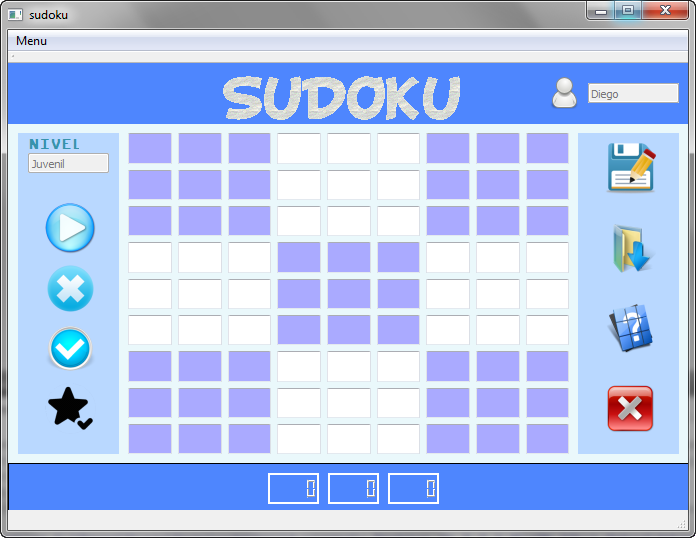
\includegraphics[width=.60\textwidth]{./imagenes/Sudoku.png}
\caption{Tablero Sudoku}
\label{Tablero Sudoku}
\end{center}
\end{figure}


\newpage
\section{Herramientas Utilizadas en el Desarrollo del Proyecto:}

\begin{figure}[htbp]
\begin{center}
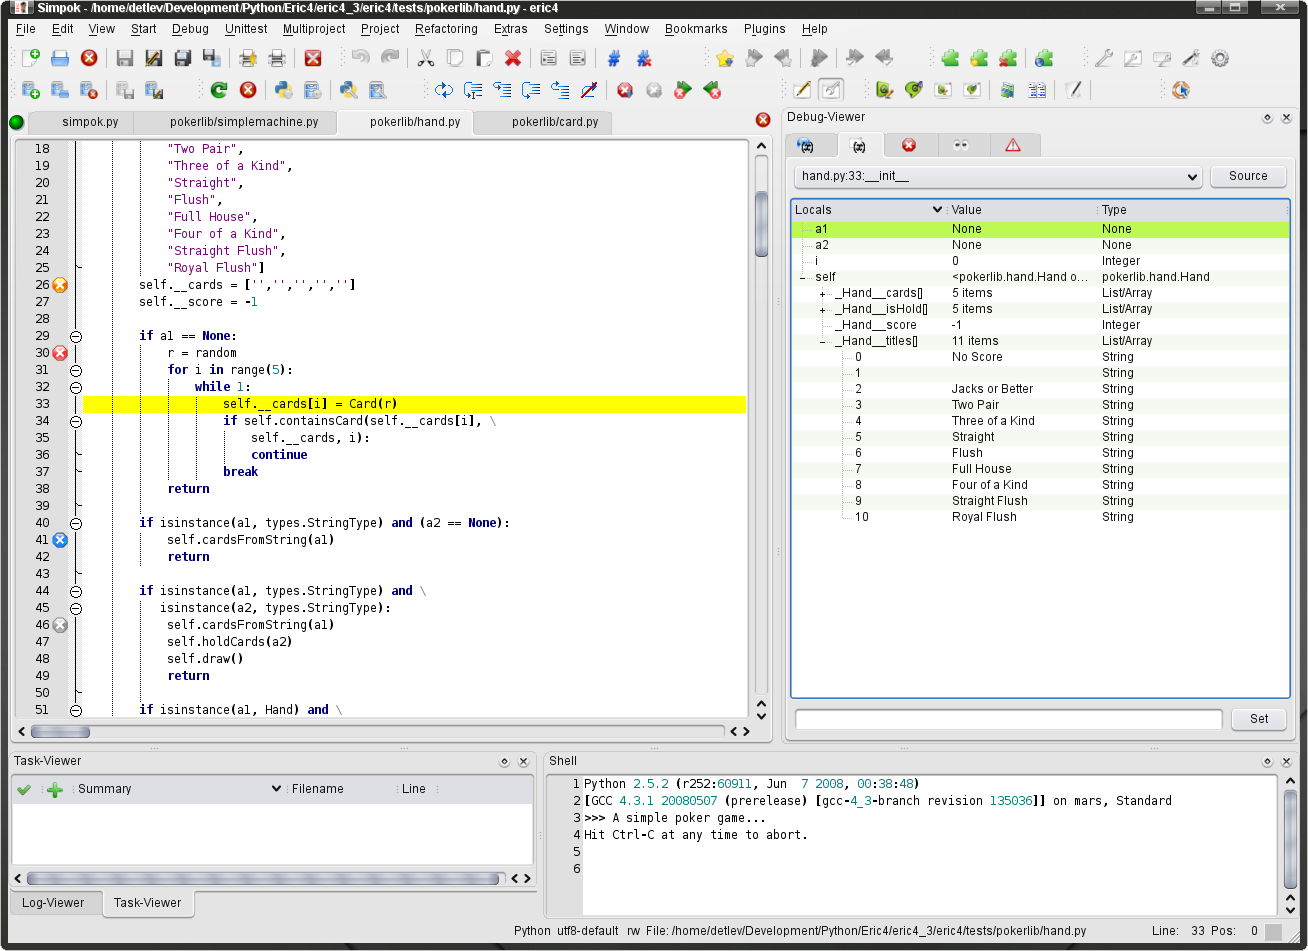
\includegraphics[width=.70\textwidth]{./imagenes/ide_python.png}
\caption{Python}
\label{Python}
\end{center}
\end{figure}

\ \\ 
Python es un lenguaje de programaci\'on interpretado cuya filosof\'\i{}a hace hincapi\'e en una sintaxis muy limpia y que favorezca un c\'odigo legible.
Se trata de un lenguaje de programaci\'on multiparadigma, ya que soporta orientaci\'on a objetos, programaci\'on imperativa y, en menor medida, programaci\'on funcional. Es un lenguaje interpretado, usa tipado din\'amico y es multiplataforma.
Es administrado por la Python Software Foundation. Posee una licencia de c\'odigo abierto, denominada Python Software Foundation License, que es compatible con la Licencia p\'ublica general de GNU a partir de la versi�n 2.1.1, e incompatible en ciertas versiones anteriores.
\ \\


\newpage
\section{GitHub:}
\begin{figure}[htbp]
\begin{center}

\includegraphics[width=.70\textwidth]{./imagenes/github_logo.jpg}
\caption{git}
\label{git}
\end{center}
\end{figure}

\ \\ 
GitHub es una forja para alojar proyectos utilizando el sistema de control de versiones Git. Utiliza el framework Ruby on Rails por GitHub, Inc. (anteriormente conocida como Logical Awesome).
Desde enero de 2010, GitHub opera bajo el nombre de GitHub, Inc.
El c\'odigo se almacena de forma publica, aunque tambi�n se puede hacer de forma privada, creando una cuenta de pago.
\ \\


\newpage
\section{Doxygen:}
\begin{figure}[htbp]
\begin{center}
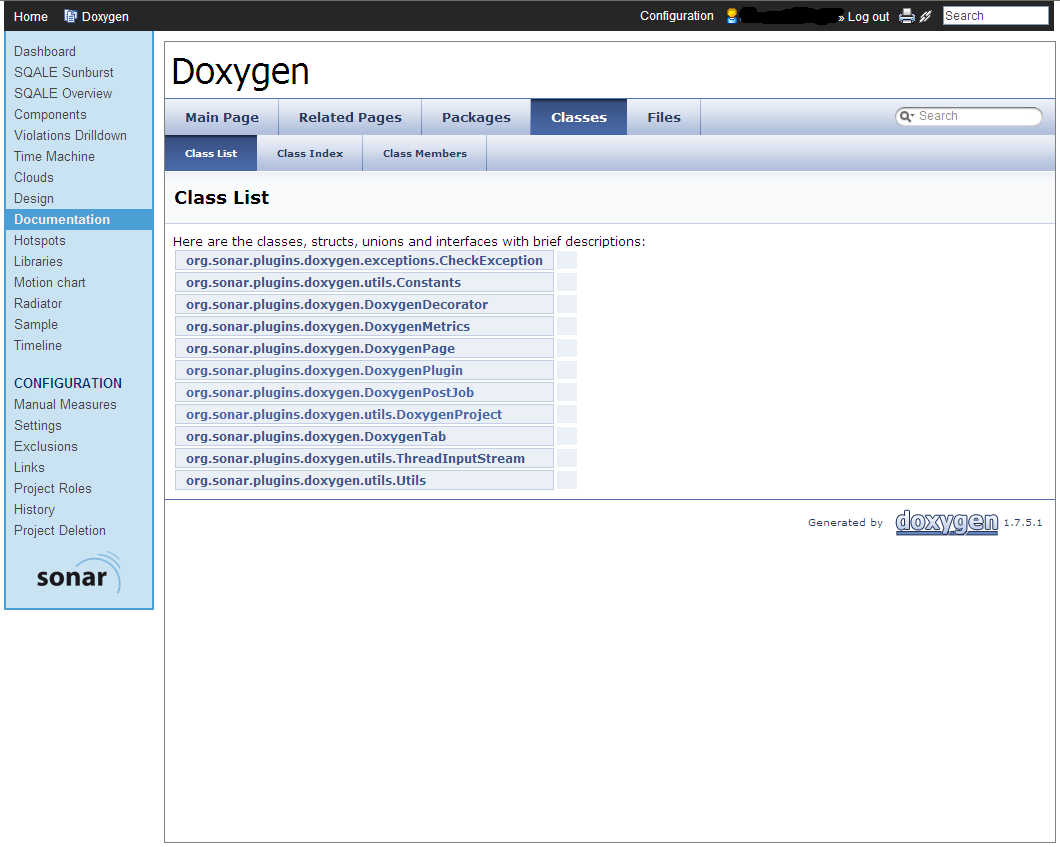
\includegraphics[width=.70\textwidth]{./imagenes/doxygen.png}
\caption{doxygen}
\label{doxygen}
\end{center}
\end{figure}
\ \\ 
Doxygen es un generador de documentaci\'on para C++, C, Java, Objective-C, Python, IDL (versiones Corba y Microsoft), VHDL y en cierta medida para PHP y D. Dado que es f\'acilmente adaptable, funciona en la mayor\'\i{}a de sistemas Unix as� como en Windows y Mac OS X. La mayor parte del c\'odigo de Doxygen esta escrita por Dimitri van Heesch.
Doxygen es un acr\'onimo de dox(document) gen(generator), generador de documentaci\'on para codigo fuente.
Varios proyectos como KDE usan Doxygen para generar la documentacion de su API. KDevelop incluye soporte para Doxygen.
\ \\

\newpage
\section{Objetivos:}
\ \\ 
Crear una aplicaci\'on de sudoku en Python.
\ \\ 
Utilizar Python como principal herramienta de desarrollo.
\ \\ 
Encontrar las ventajas que ofrece Python en comparaci\'on a otros lenguajes antes ulitlizados.
\ \\ 
Implementar la aplicaci\'on con la metodolog\'\i{}a Orientada a objetos en Python.
\ \\ 
Utilizar GIT como herramienta de control de versionamiento.
\ \\ 
Utilizar Doxygen para documentacion del c\'odigo.
\ \\

\section{Desarrollo:}
\ \\ 
El desarrollo de este segundo proyecto se realiz\'o entre dos integrantes del grupo, empezando por crear la interfaz de la aplicaci\'on, que se logr\'o hacerlo importando la interfaz utilizada en QT a Python, luego de esto se procedio a implementar la funcionalidad investigando la sintaxis del Lenguaje para el paso de la funcionalidad de QT a Python.

El trabajo fue dividido entre los dos integrantes del grupo,  Carlos Ram\'\{}irez desarrollo parte de la funcionalidad de las pistas, correcci\'on ingame del sudoku de los n\'umeros ingresados en el tablero por medio del evento textChanged y de la opci\'on de dar pista que permit\'\i{}a mostrar al usuario que valor ingresado era correcto y cual no lo era antes de terminar de llenar el tablero, optimizar ciertas partes del c\'odigo como el momento de generar tableros y la documentaci\'on de la aplicaci\'on. 

Jos\'e V\'elez desarrollo el iniciar partida el cual generaba tableros a partir de una plantilla otra de las funcionalidades implementadas fue el cargar y guardar partida, debidamente encriptado con operaciones de desplazamiento y operaciones aritmeticas al c\'odigo ASCII de los valores del tablero de sudoku. Tambi\'en se encargo de implementar los puntajes que se calculaba en base al tiempo tomado en resolver el juego.

\ \\

\newpage
\section{Conclusiones:}
\ \\ 
La experiencia en Python, como herramienta de trabajo fue satisfactoria debido a que se orientaba a objetos tenia similitudes al lenguaje java, el inconveniente fue el poco tiempo para aprender a manejar la herramienta,una de las ventajas encontradas es que Python es un lenguaje de c\'odigo mejor estructurado por su organizaci\'on por identaci\'on, con la particularidad que no se necesita declarar el tipo de variable, entre las ventajas de Python encontramos, su compatibilidad debido a ser un lenguaje interpretado, una de las desventajas podr\'\i{}a ser un poco menos eficiente en cuestion de tiempo de ejecuci\'on ya que al ser un lenguaje interpretado consume mas recursos que un lenguaje compilado.
\ \\ 
\section{Referencias:}
\ \\ 

	http://mundogeek.net/tutorial-python/

\ \\ 

	http://docs.python.org/2/tutorial/
	
\ \\ 

	http://www.python.org/doc/
	
\ \\ 
\newpage






\end{document}  
